\documentclass{standalone}
\usepackage{tikz}
\usetikzlibrary{patterns, positioning}

\begin{document}
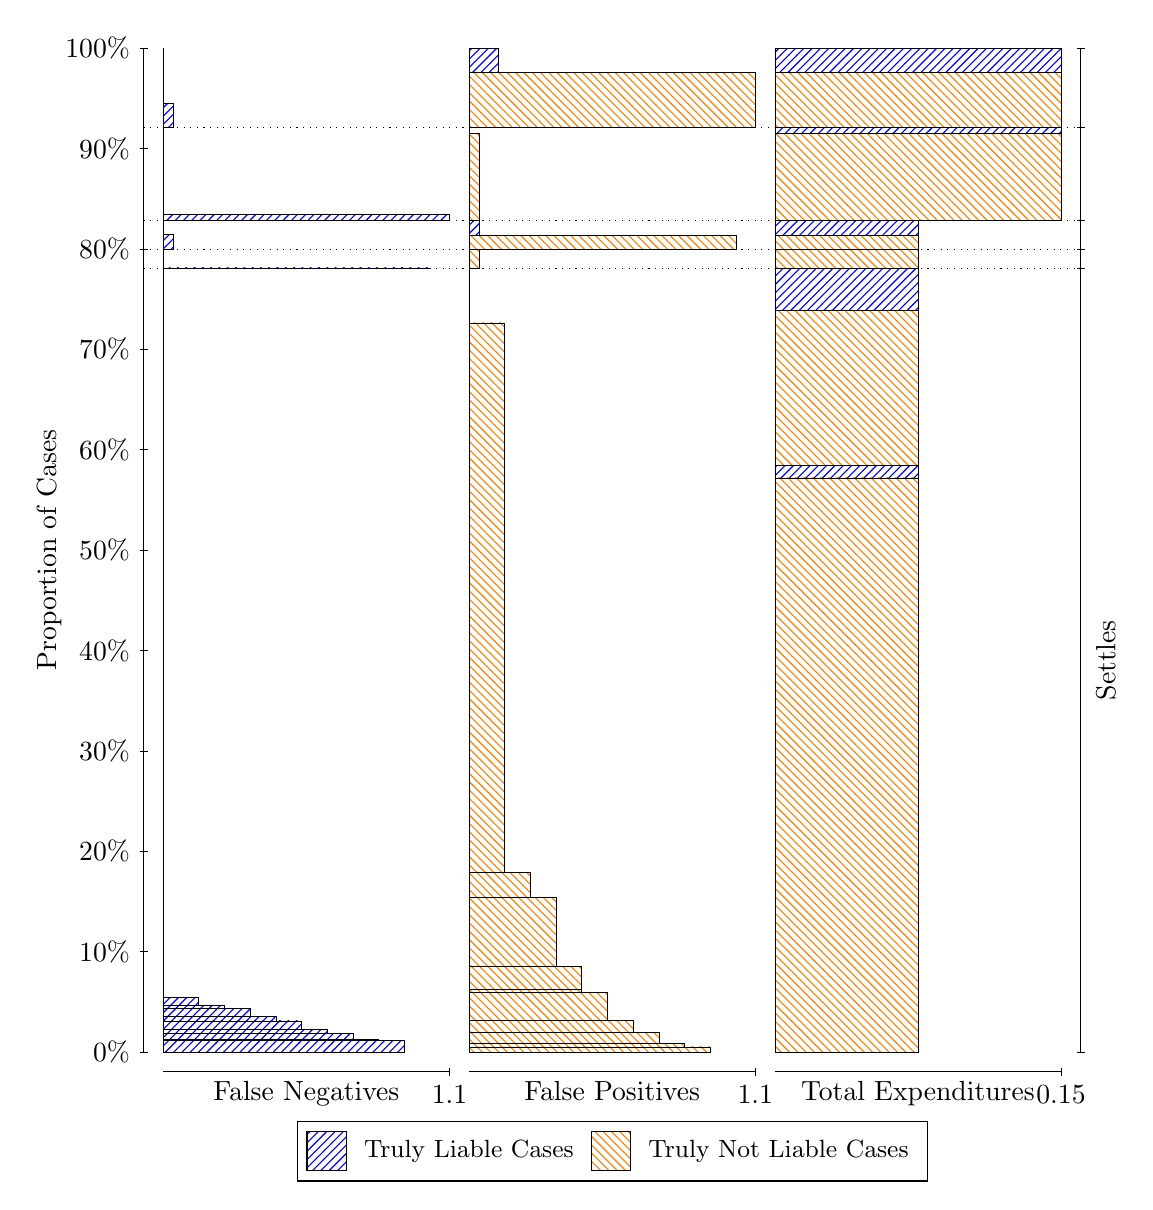
\begin{tikzpicture}
\draw[black, very thin] (1.5,1.75) -- (1.5,14.5);
\node[rotate=90, anchor=center] at (0.3, 8.125) {Proportion of Cases};
\draw[black, very thin] (1.45,1.75) -- (1.55,1.75);
\node[anchor=east] at (1.45, 1.75) {0\%};
\draw[black, very thin] (1.45,3.025) -- (1.55,3.025);
\node[anchor=east] at (1.45, 3.025) {10\%};
\draw[black, very thin] (1.45,4.3) -- (1.55,4.3);
\node[anchor=east] at (1.45, 4.3) {20\%};
\draw[black, very thin] (1.45,5.575) -- (1.55,5.575);
\node[anchor=east] at (1.45, 5.575) {30\%};
\draw[black, very thin] (1.45,6.85) -- (1.55,6.85);
\node[anchor=east] at (1.45, 6.85) {40\%};
\draw[black, very thin] (1.45,8.125) -- (1.55,8.125);
\node[anchor=east] at (1.45, 8.125) {50\%};
\draw[black, very thin] (1.45,9.4) -- (1.55,9.4);
\node[anchor=east] at (1.45, 9.4) {60\%};
\draw[black, very thin] (1.45,10.675) -- (1.55,10.675);
\node[anchor=east] at (1.45, 10.675) {70\%};
\draw[black, very thin] (1.45,11.95) -- (1.55,11.95);
\node[anchor=east] at (1.45, 11.95) {80\%};
\draw[black, very thin] (1.45,13.225) -- (1.55,13.225);
\node[anchor=east] at (1.45, 13.225) {90\%};
\draw[black, very thin] (1.45,14.5) -- (1.55,14.5);
\node[anchor=east] at (1.45, 14.5) {100\%};

\draw[black, very thin] (13.4,1.75) -- (13.4,14.5);
\draw[black, very thin] (13.35,1.75) -- (13.45,1.75);
\node[anchor=west] at (13.35, 1.75) {};
\draw[black, very thin] (13.35,11.702) -- (13.45,11.702);
\node[anchor=west] at (13.35, 11.702) {};
\draw[black, very thin] (13.35,11.946) -- (13.45,11.946);
\node[anchor=west] at (13.35, 11.946) {};
\draw[black, very thin] (13.35,12.314) -- (13.45,12.314);
\node[anchor=west] at (13.35, 12.314) {};
\draw[black, very thin] (13.35,13.49) -- (13.45,13.49);
\node[anchor=west] at (13.35, 13.49) {};
\draw[black, very thin] (13.35,14.5) -- (13.45,14.5);
\node[anchor=west] at (13.35, 14.5) {};

\draw[black, very thin, pattern color=blue, pattern=north east lines] (1.75,1.75) rectangle (4.8118,1.8934);
\draw[black, very thin, pattern color=blue, pattern=north east lines] (1.75,1.8934) rectangle (4.4852,1.9081);
\draw[black, very thin, pattern color=blue, pattern=north east lines] (1.75,1.9081) rectangle (4.1586,1.9852);
\draw[black, very thin, pattern color=blue, pattern=north east lines] (1.75,1.9852) rectangle (3.832,2.0351);
\draw[black, very thin, pattern color=blue, pattern=north east lines] (1.75,2.0351) rectangle (3.5054,2.1444);
\draw[black, very thin, pattern color=blue, pattern=north east lines] (1.75,2.1444) rectangle (3.1788,2.2021);
\draw[black, very thin, pattern color=blue, pattern=north east lines] (1.75,2.2021) rectangle (2.8522,2.2987);
\draw[black, very thin, pattern color=blue, pattern=north east lines] (1.75,2.2987) rectangle (2.5257,2.3448);
\draw[black, very thin, pattern color=blue, pattern=north east lines] (1.75,2.3448) rectangle (2.1991,2.4436);
\draw[black, very thin, pattern color=orange, pattern=north west lines] (1.75,2.4436) rectangle (1.75,11.702);
\draw[black, very thin, pattern color=blue, pattern=north east lines] (1.75,11.702) rectangle (5.1384,11.708);
\draw[black, very thin, pattern color=orange, pattern=north west lines] (1.75,11.708) rectangle (1.75,11.946);
\draw[black, very thin, pattern color=blue, pattern=north east lines] (1.75,11.946) rectangle (1.8725,12.135);
\draw[black, very thin, pattern color=orange, pattern=north west lines] (1.75,12.135) rectangle (1.75,12.314);
\draw[black, very thin, pattern color=blue, pattern=north east lines] (1.75,12.314) rectangle (5.3833,12.391);
\draw[black, very thin, pattern color=orange, pattern=north west lines] (1.75,12.391) rectangle (1.75,13.49);
\draw[black, very thin, pattern color=blue, pattern=north east lines] (1.75,13.49) rectangle (1.8725,13.8);
\draw[black, very thin, pattern color=orange, pattern=north west lines] (1.75,13.8) rectangle (1.75,14.5);
\draw[black, very thin, pattern color=orange, pattern=north west lines] (5.6333,1.75) rectangle (8.6951,1.8141);
\draw[black, very thin, pattern color=orange, pattern=north west lines] (5.6333,1.8141) rectangle (8.3685,1.8576);
\draw[black, very thin, pattern color=orange, pattern=north west lines] (5.6333,1.8576) rectangle (8.0419,2.0037);
\draw[black, very thin, pattern color=orange, pattern=north west lines] (5.6333,2.0037) rectangle (7.7154,2.1471);
\draw[black, very thin, pattern color=orange, pattern=north west lines] (5.6333,2.1471) rectangle (7.3888,2.5071);
\draw[black, very thin, pattern color=orange, pattern=north west lines] (5.6333,2.5071) rectangle (7.0622,2.5453);
\draw[black, very thin, pattern color=orange, pattern=north west lines] (5.6333,2.5453) rectangle (7.0622,2.8368);
\draw[black, very thin, pattern color=orange, pattern=north west lines] (5.6333,2.8368) rectangle (6.7356,3.7172);
\draw[black, very thin, pattern color=orange, pattern=north west lines] (5.6333,3.7172) rectangle (6.409,4.0302);
\draw[black, very thin, pattern color=orange, pattern=north west lines] (5.6333,4.0302) rectangle (6.0824,11.008);
\draw[black, very thin, pattern color=blue, pattern=north east lines] (5.6333,11.008) rectangle (5.6333,11.702);
\draw[black, very thin, pattern color=orange, pattern=north west lines] (5.6333,11.702) rectangle (5.7558,11.94);
\draw[black, very thin, pattern color=blue, pattern=north east lines] (5.6333,11.94) rectangle (5.6333,11.946);
\draw[black, very thin, pattern color=orange, pattern=north west lines] (5.6333,11.946) rectangle (9.0217,12.125);
\draw[black, very thin, pattern color=blue, pattern=north east lines] (5.6333,12.125) rectangle (5.7558,12.314);
\draw[black, very thin, pattern color=orange, pattern=north west lines] (5.6333,12.314) rectangle (5.7558,13.413);
\draw[black, very thin, pattern color=blue, pattern=north east lines] (5.6333,13.413) rectangle (5.6333,13.49);
\draw[black, very thin, pattern color=orange, pattern=north west lines] (5.6333,13.49) rectangle (9.2667,14.19);
\draw[black, very thin, pattern color=blue, pattern=north east lines] (5.6333,14.19) rectangle (6.0007,14.5);
\draw[black, very thin, pattern color=orange, pattern=north west lines] (9.5167,1.75) rectangle (11.333,9.041);
\draw[black, very thin, pattern color=blue, pattern=north east lines] (9.5167,9.041) rectangle (11.333,9.199);
\draw[black, very thin, pattern color=orange, pattern=north west lines] (9.5167,9.199) rectangle (11.333,11.166);
\draw[black, very thin, pattern color=blue, pattern=north east lines] (9.5167,11.166) rectangle (11.333,11.702);
\draw[black, very thin, pattern color=orange, pattern=north west lines] (9.5167,11.702) rectangle (11.333,11.94);
\draw[black, very thin, pattern color=blue, pattern=north east lines] (9.5167,11.94) rectangle (11.333,11.946);
\draw[black, very thin, pattern color=orange, pattern=north west lines] (9.5167,11.946) rectangle (11.333,12.125);
\draw[black, very thin, pattern color=blue, pattern=north east lines] (9.5167,12.125) rectangle (11.333,12.314);
\draw[black, very thin, pattern color=orange, pattern=north west lines] (9.5167,12.314) rectangle (13.15,13.413);
\draw[black, very thin, pattern color=blue, pattern=north east lines] (9.5167,13.413) rectangle (13.15,13.49);
\draw[black, very thin, pattern color=orange, pattern=north west lines] (9.5167,13.49) rectangle (13.15,14.19);
\draw[black, very thin, pattern color=blue, pattern=north east lines] (9.5167,14.19) rectangle (13.15,14.5);
\draw[black, dotted] (1.5,11.702) -- (13.4,11.702);
\draw[black, dotted] (1.5,11.946) -- (13.4,11.946);
\draw[black, dotted] (1.5,12.314) -- (13.4,12.314);
\draw[black, dotted] (1.5,13.49) -- (13.4,13.49);
\draw[black, very thin] (1.75,1.5) -- (5.3833,1.5);
\node[anchor=north] at (3.5667, 1.5) {False Negatives};
\draw[black, very thin] (5.3833,1.45) -- (5.3833,1.55);
\node[anchor=north] at (5.3833, 1.45) {1.1};

\draw[black, very thin] (5.6333,1.5) -- (9.2667,1.5);
\node[anchor=north] at (7.45, 1.5) {False Positives};
\draw[black, very thin] (9.2667,1.45) -- (9.2667,1.55);
\node[anchor=north] at (9.2667, 1.45) {1.1};

\draw[black, very thin] (9.5167,1.5) -- (13.15,1.5);
\node[anchor=north] at (11.333, 1.5) {Total Expenditures};
\draw[black, very thin] (13.15,1.45) -- (13.15,1.55);
\node[anchor=north] at (13.15, 1.45) {0.15};

\node[black, centered, rotate=90] at (13.72, 6.7259) {Settles};





\draw (7.449999999999999,1.5) node[draw=none] (baseCoordinate) {};
\begin{scope}[align=center]
        \matrix[scale=0.5, draw=black, below=0.5cm of baseCoordinate, nodes={draw}, column sep=0.1cm]{
            \node[rectangle, draw, minimum width=0.5cm, minimum height=0.5cm, pattern=north east lines, pattern color=blue] {}; &
            \node[draw=none, font=\small] (B) {Truly Liable Cases}; &
            \node[rectangle, draw, minimum width=0.5cm, minimum height=0.5cm, pattern=north west lines, pattern color=orange] {}; &
            \node[draw=none, font=\small] (B) {Truly Not Liable Cases}; \\
            };
\end{scope}

\end{tikzpicture}
\end{document}